\chapter{СИСТЕМИЙН ШИНЖИЛГЭЭ}

\section{Оролцогч талууд}

Энэхүү системийн үндсэн хэрэглэгч нь оюутан боловч системийн бүрэн хэрэглээнд багш, удирдагч, сургуулийн системийн администратор, мөн MCP-ээр холбогдох бусад системийн орчин нөлөөлнө.

Оюутан нь системийн гол хэрэглэгч бөгөөд хуваарь, дүн, мэдэгдэл, баримт бичиг, даалгаврын мэдээллийг хурдан авах, дахин нэвтрэлтгүйгээр өдөр тутмын ажлаа автоматжуулах сонирхолтой. Багш нь багшийн порталтай холбогдсон үед дүн оруулах, ялангуяа Excel файлаас олон оюутны дүнг хялбар оруулах зэрэг ажлыг автоматжуулахыг хүсдэг. Удирдагч багш болон комисс нь системийн судалгааны үндэслэл, архитектурын зөв байдал, хэрэгжих боломж, ахицыг үнэлэх үүрэгтэй. Сургуулийн системийн орчин нь порталын нэвтрэлт, API өөрчлөлт, өгөгдлийн бодит байдал, аюулгүй байдлын шаардлагыг тодорхойлно. Бусад MCP үйлчилгээнүүд нь ирээдүйд холбогдох календарь, баримт бичиг, өгөгдөл экспорт, бусад автоматжуулалтын интеграцын боломжийг бүрдүүлнэ.

\section{Ашиглалтын хувилбарууд}

Системийн гол ашиглалтын хувилбаруудыг Зураг~\ref{fig:usecases}-д нэгтгэн үзүүлэв. Эдгээр use case-үүдийг одоогийн хэрэгжилтийн төлөвийн хамт Хүснэгт~\ref{tab:usecases}-д тайлбарлав.

\begin{figure}[H]
  \centering
  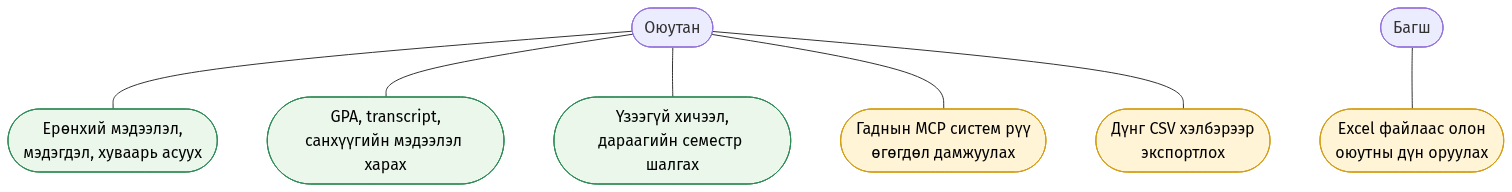
\includegraphics[width=0.95\textwidth]{assets/diagrams/usecases.png}
  \caption{SISi Intelligent Agent-ын үндсэн ашиглалтын хувилбарууд}
  \label{fig:usecases}
\end{figure}

% ШИНЭ ДИАГРАМ ХЭРЭГТЭЙ: Use case диаграмыг шинэчлэх. Оюутан болон Багш гэсэн хоёр actor-той, 
% UC-1-ээс UC-8 хүртэлх use case-үүдийг харуулсан UML use case диаграм.
% Оюутан: UC-1 (Ерөнхий мэдээлэл), UC-2 (Хуваарь), UC-3 (Дүн/GPA), UC-4 (E-journal), 
%         UC-5 (MCP интеграц), UC-6 (CSV export)
% Багш: UC-7 (Excel-ээс дүн оруулах), UC-8 (Баталгаажуулалт)
% Нийтлэг: Session bootstrap

\begin{table}[H]
  \centering
  \caption{Үндсэн use case-үүд ба тэдгээрийн төлөв}
  \label{tab:usecases}
  \begin{tabularx}{\textwidth}{>{\raggedright\arraybackslash}p{1cm} >{\raggedright\arraybackslash}X >{\raggedright\arraybackslash}p{3cm}}
    \toprule
    № & Тодорхойлолт & Төлөв \\
    \midrule
    UC-1 & Оюутны ерөнхий мэдээлэл, идэвхтэй хичээлүүд, порталын мэдэгдлийг байгалийн хэлээр асууж авах & MCP tool бэлэн \\
    UC-2 & Хичээлийн болон шалгалтын хуваарийг асууж авах, тодорхой өдөр эсвэл долоо хоногоор шүүх & MCP tool бэлэн \\
    UC-3 & Дүн, GPA, transcript, кредитийн мэдээллийг харах, шинжлэх & MCP tool бэлэн \\
    UC-4 & E-journal-ийн мэдээлэл, үнэлгээний бүрэлдэхүүн хэсгүүдийг харах & Хэсэгчлэн бэлэн \\
    UC-5 & Порталын өгөгдлийг MCP-ээр холбогдсон гаднын системүүд рүү (календарь, todo app) дамжуулах & Төлөвлөсөн \\
    UC-6 & Дүн, хуваарь зэрэг өгөгдлийг CSV эсвэл бусад форматаар экспортлох & Төлөвлөсөн \\
    UC-7 & Багшийн порталын API ашиглан Excel файлаас олон оюутны дүн оруулах & Төлөвлөсөн \\
    UC-8 & Эрсдэлтэй үйлдэл (mutation) хийхээс өмнө хэрэглэгчээс баталгаажуулалт авах & Төлөвлөсөн \\
    \bottomrule
  \end{tabularx}
\end{table}

UC-1-ээс UC-3 хүртэлх use case-үүд нь MCP серверт бүрэн хэрэгжсэн бөгөөд SISI API-гаас оюутны үндсэн мэдээлэл, хуваарь, дүн, санхүүгийн мэдээллийг амжилттай уншиж байна. UC-4 нь e-journal хэсгийн зарим API хязгаарлалтаас болж хэсэгчлэн хэрэгжсэн. UC-5-аас UC-8 хүртэлх use case-үүд нь дараагийн шатанд хэрэгжих төлөвлөгөөтэй.

\section{Функциональ шаардлага}

Системийн функциональ шаардлагыг дараах байдлаар тодорхойлов.

\subsection{Хэрэглэгчийн оролт ба гаралт}

Хэрэглэгч Chrome extension-оор дамжуулан байгалийн хэлээр асуулт, даалгавар өгөх боломжтой байх ёстой. Систем нь хэрэглэгчийн хүсэлтийг ойлгож, шаардлагатай мэдээллийг цуглуулж, ойлгомжтой текст хэлбэрээр хариулах чадвартай байна. Хариулт нь зөвхөн түүхий өгөгдөл бус, хэрэглэгчид ойлгомжтой тайлбар, дүгнэлт агуулсан байх ёстой.

\subsection{Өгөгдөлд хандалт}

Систем нь оюутны идэвхтэй сесс дээр тулгуурлан SISI API-гаас бодит өгөгдөл унших чадвартай байна. Хэрэглэгчийг дахин нэвтрүүлэхгүйгээр тухайн порталаас авсан access token эсвэл холбогдох сессийн мэдээллийг аюулгүй бүртгэдэг байх шаардлагатай. Хуваарь, дүн, санхүү, мэдэгдэл, баримт бичиг, e-journal зэрэг үндсэн домэйнүүдийг тусдаа MCP хэрэгслээр дуудах боломжтой байна.

\subsection{Өргөтгөх чадвар}

Систем нь ирээдүйд дурын MCP нийцтэй гаднын үйлчилгээ болон багшийн порталын API-тай холбогдох өргөтгөх чадвартай байх ёстой. Шинэ хэрэгсэл нэмэхэд бүх системийг дахин бичих шаардлагагүй байх модульчлагдсан бүтэцтэй байна.

\subsection{Аюулгүй байдал}

Экспорт, submit зэрэг mutation үйлдэлд хэрэглэгчээс баталгаажуулалт шаардах механизмтай байна. Хэрэглэгчийн session-id, хугацаа дуусах төлөв, зөвшөөрөгдсөн origin-уудыг удирдах чадвартай байх шаардлагатай. Read-only болон mutation хэрэгслүүдийг тодорхой ялгаж, mutation-д нэмэлт хяналт тавина.

\section{Функциональ бус шаардлага}

\subsection{Аюулгүй байдал}

Систем нь нэвтрэх мэдээллийг ил хадгалахгүй байх ёстой. Локал сессийн хугацааг хязгаарлаж (idle TTL), зөвшөөрөгдсөн origin ашиглах замаар аюулгүй байдлыг хангана. Access token болон cookie-г AI загварт шууд ил гаргахгүй, зөвхөн MCP серверээр дамжуулан хэрэглэнэ.

\subsection{Өргөтгөх чадвар}

Шинэ MCP домэйн, шинэ гадаад интеграц, шинэ client төрлүүдийг бага өөрчлөлтөөр нэмэх боломжтой байна. Модульчлагдсан архитектур нь бүрэлдэхүүн хэсгүүдийг бие даан хөгжүүлэх, туршихад тохиромжтой.

\subsection{Найдвартай байдал}

Upstream API алдаа гарсан тохиолдолд систем нь ойлгомжтой алдааны мэдэгдэл буцаах ёстой. Хэрэглэгчид юу болсныг мэдэгдэж, шаардлагатай бол дахин оролдох боломж олгоно.

\subsection{Гүйцэтгэл}

Энгийн унших хүсэлтүүдийг боломжит богино хугацаанд гүйцэтгэх ёстой. MCP серверийн хариу хугацаа нь upstream API-ийн хариу хугацаанаас хамаарах боловч нэмэлт саатал хамгийн бага байх ёстой.

\subsection{Хянах боломж}

Аль хэрэгсэл ямар өгөгдөл ашигласныг тайлбарлах боломжтой байна. Mutation үйлдлүүдийн түүх, лог бичлэг хадгалагдах ёстой.

\subsection{Хэрэглэх боломж}

Порталд аль хэдийн нэвтэрсэн хэрэглэгч нэмэлт нэвтрэлтгүйгээр системийг ашиглахад ойлгомжтой байх ёстой. Байгалийн хэлний интерфейс нь техникийн мэдлэг шаардахгүй, энгийн хүмүүст хүртээмжтэй байна.

\section{Эрсдэл ба хязгаарлалт}

Завсрын шатанд хэд хэдэн эрсдэл, хязгаарлалт ажиглагдаж байна.

SISI порталын API нь албан ёсны тогтвортой public contract биш байж болох тул ирээдүйд өөрчлөлт гарч болзошгүй. Энэ тохиолдолд MCP серверийн upstream client-ийг шинэчлэх шаардлагатай болно. Гэхдээ модульчлагдсан архитектур нь энэ өөрчлөлтийг бусад бүрэлдэхүүнүүдэд нөлөөлөхгүйгээр хийх боломжийг олгоно.

Бичих үйлдэлтэй холбоотой submit, export, state change төрлийн функцуудыг шууд нээх нь аюулгүй байдлын нэмэлт шалгалт шаарддаг. Буруу хэрэглэгч эсвэл буруу ойлгосон команд нь санамсаргүй өөрчлөлт хийх эрсдэлтэй тул баталгаажуулалтын давхарга заавал хэрэгтэй.

Хиймэл оюуны загварын тайлбарлал буруу байвал буруу хэрэгсэл дуудах эрсдэлтэй. Жишээлбэл, ``миний дүн'' гэж асуухад санхүүгийн дүн буцаах зэрэг алдаа гарч болно. Иймд tool routing-ийн логик, хэрэгслийн тодорхойлолт, загварын prompt зэргийг сайтар загварчлах шаардлагатай.

Олон төрлийн MCP үйлчилгээ болон багшийн порталын mutation урсгал нэмэгдэхэд зөвшөөрөл, аудит, алдаа шалгалтын төвөгшил өсөх болно. Энэ нь архитектурын цэвэр байдал, баримт бичгийн чанар, туршилтын хамрах хүрээг улам чухал болгоно.
